\documentclass[conference]{IEEEtran}
\IEEEoverridecommandlockouts
\usepackage{cite}
\usepackage{amsmath,amssymb,amsfonts}
\usepackage{algorithmic}
\usepackage{graphicx}
\usepackage{textcomp}
\usepackage{xcolor}
\usepackage{booktabs}
\usepackage{multirow}
\usepackage{url}
\usepackage{hyperref}
\hypersetup{colorlinks=true, citecolor=blue, urlcolor=blue}

\title{Foundation Models versus Engineered-Feature Linear Regression for Vietnamese Gold Price Forecasting under Regime Shifts}

\author{
\IEEEauthorblockN{WangNhat\IEEEauthorrefmark{1}}
\IEEEauthorblockA{
\IEEEauthorrefmark{1}Faculty of Information Technology, Ton Duc Thang University, Vietnam \\
Email: dev2@wolffungame.com
}
}

\begin{document}
\maketitle

\begin{abstract}
We benchmark 27 forecasting models---spanning classical statistical, tabular machine learning, deep learning, regime-aware ensembles, and zero-shot foundation models---on the Vietnamese SJC physical gold market across three horizons ($h\in\{1,5,20\}$ days). Using walk-forward cross-validation with 5 expanding-window folds and the Friedman--Nemenyi non-parametric test, we find that \emph{regularized linear regression} (Ridge / ElasticNet) on 116 engineered features (lag, returns, technical, macro, calendar, sentiment) consistently outperforms more complex tree, RNN, and Transformer architectures, achieving MAPE of $0.63\%$, $1.41\%$, and $3.06\%$ for $h=1,5,20$ respectively---an order of magnitude better than the proposal target of $4$--$5\%$. The Amazon Chronos-Bolt-Small foundation model, applied zero-shot without any training data, attains $3.07\%$ MAPE at $h=1$, competitive with classical baselines. Friedman tests reject equal-accuracy at $p<10^{-3}$ for all horizons. A cumulative feature-family ablation shows that technical indicators contribute the largest single-family gain at $h=1$ ($-0.34$\,pp MAPE), while sentiment lags from a $400$-headline mDeBERTa pipeline have negligible impact in the current evaluation window---a faithfully-reported limitation due to historical news-archive coverage gaps. We further demonstrate Adaptive Conformal Inference (ACI) maintaining $86\%$ marginal coverage at $h=1$ versus $76\%$ for vanilla split conformal during the 2024 SJC rally regime shift, where in fold~3 split coverage collapses to $9\%$ while ACI holds above $80\%$. SHAP analysis confirms lag dominance, but macro variables (USD index, 10-year Treasury, GLD ETF) appear consistently among the top 20. All code, data, leaderboards, ablation, conformal results, a Streamlit / PWA dashboard, FastAPI service, Telegram bot, weekly retraining pipeline, and Docker images are released under the MIT licence.
\end{abstract}

\begin{IEEEkeywords}
gold price forecasting, foundation models, conformal prediction, walk-forward cross-validation, ablation study, Vietnam, SJC, time series, regime shift
\end{IEEEkeywords}

\section{Introduction}

The Vietnamese physical gold market (vàng miếng SJC) exhibits a persistent premium of $10$--$15\%$ over international spot gold, driven by domestic supply--demand dynamics, USD/VND fluctuations, and limited cross-border arbitrage \cite{bouteska2023}. This premium causes regime shifts: during the 2024 gold rally, SJC prices surged from $\sim$75 to $\sim$95 million VND per tael, deviating sharply from international gold trends. Accurate and risk-calibrated forecasting under such regime shifts is critical for retail investors, gold-trading enterprises, and the central bank for market surveillance.

Despite a recent surge in time-series foundation models (Chronos \cite{ansari2024chronos}, TimesFM \cite{das2024timesfm}, Moirai, TTM \cite{ekambaram2024ttm}, Lag-Llama \cite{rasul2024laglama}) and SOTA Transformers (PatchTST \cite{nie2023patchtst}, iTransformer \cite{liu2024itransformer}, TFT \cite{lim2021tft}), no systematic benchmark exists for the SJC market. This work addresses four research questions:

\begin{enumerate}
\item How do foundation models (zero-shot) compare against trained tabular ML and deep learning on a small ($\sim$2{,}000 observations), volatile, emerging-market asset?
\item Which feature \emph{families} (lag, returns, technical, macro, calendar, sentiment) drive predictive accuracy, and what is the marginal contribution of each?
\item Does Adaptive Conformal Inference (ACI) \cite{gibbs2021aci} maintain coverage validity during the 2024 SJC regime shift compared to split conformal \cite{vovk2005}, across multiple horizons and base learners?
\item Can lightweight regime-aware ensembles outperform a single global model when the volatility regime is detected with simple statistical thresholds?
\end{enumerate}

Our contributions:
\begin{itemize}
\item A reproducible pipeline benchmarking 27 forecasting models across 3 horizons on 8 years of SJC data, with rigorous walk-forward cross-validation and Friedman--Nemenyi statistical tests (420 model--fold--horizon records).
\item Empirical evidence that regularized linear regression on 116 engineered features outperforms all tree-based, deep learning, and foundation models on this dataset---and a cumulative feature-family ablation that quantifies the marginal contribution of each family.
\item First demonstration of Chronos-Bolt zero-shot competitive performance on Vietnamese gold ($3.07\%$ MAPE, $h=1$) without any fine-tuning.
\item Per-fold ACI conformal coverage analysis under regime shift across 3 horizons and 3 base learners (Ridge, ElasticNet, LightGBM), showing where vanilla split conformal collapses ($9\%$ coverage in fold~3 at $h=1$) and where ACI retains target coverage ($\geq 80\%$).
\item A complete free-tier productisation stack---Streamlit dashboard with PWA installability, FastAPI inference service, Telegram bot, weekly automated retraining via GitHub Actions cron, and Docker Compose deployment---released under MIT license at \url{https://github.com/twangnhat-05/NGHIENCUUKHOAHOC}.
\end{itemize}

\section{Related Work}

\subsection{Vietnamese gold price forecasting}
Bouteska et al.\ \cite{bouteska2023} apply time-varying parameter VAR to SJC during COVID-19. Dao \cite{dao2024} explores correlation between SJC and macro variables. Ha and Tran \cite{ha2023var} use VAR to identify macro impact. Tuan et al.\ \cite{tuan2024ensemble} apply ensemble learning. Nguyen et al.\ \cite{nguyen2025} compare classical ML on a domestic gold dataset. None of these benchmark modern foundation models, perform feature-family ablation, or assess prediction-interval validity under regime shift with multiple-comparison tests.

\subsection{Foundation models for time series}
Chronos \cite{ansari2024chronos} tokenises real-valued time series and applies T5-style pretraining on a large corpus; the Bolt variant offers $\sim$$250\times$ inference speed-up with similar accuracy. TimesFM \cite{das2024timesfm} (Google) uses a decoder-only architecture pretrained on 100B time-points. Moirai (Salesforce) and TTM \cite{ekambaram2024ttm} (IBM) target multivariate and CPU-efficient inference respectively. Lag-Llama \cite{rasul2024laglama} adopts a probabilistic decoder approach. Zero-shot evaluation on emerging-market assets remains under-explored.

\subsection{Conformal prediction under distribution shift}
Vovk's split conformal \cite{vovk2005} guarantees marginal coverage under exchangeability. ACI \cite{gibbs2021aci} adapts the miscoverage rate online via $\alpha_t = \alpha_{t-1} + \gamma(\alpha_{\text{target}} - \mathbb{1}[y_t \notin C_t])$, providing finite-sample bounded miscoverage even under distribution shift. Conformal PID \cite{angelopoulos2024conformalpid} extends this to longer-horizon dependencies---potential future work for $h=20$.

\subsection{Multilingual sentiment for Vietnamese financial news}
PhoBERT \cite{nguyen2020phobert} provides a Vietnamese-specific encoder; mDeBERTa-v3 \cite{he2023mdeberta} offers strong zero-shot multilingual classification. We use the latter to score $\sim$400 financial headlines across CafeF, VnExpress, and TinhTe, motivated by the absence of labelled VN gold-news corpora.

\section{Methodology}

\subsection{Data}
We collect 11 free-tier data sources spanning 2018-01-01 to 2026-04-25 (Table~\ref{tab:datasources}).

\begin{table}[t]
\caption{Data Sources (all free-tier)}
\label{tab:datasources}
\centering
\small
\begin{tabular}{lll}
\toprule
Source & Frequency & Provider \\
\midrule
SJC mua/bán & Daily & webgia.com (scrape) \\
Gold Futures (GC=F) & Daily & yfinance \\
USD Index (DX-Y, DTWEXBGS) & Daily & yfinance + FRED \\
VN-Index (VNINDEX) & Daily & vnstock VCI \\
Oil WTI (CL=F) & Daily & yfinance \\
FED funds rate (FEDFUNDS) & Monthly & FRED \\
10y Treasury (DGS10) & Daily & FRED \\
USD/VND (VND=X) & Daily & yfinance \\
GLD ETF & Daily & yfinance \\
BTC-USD & Daily & yfinance \\
News headlines & Daily (subset) & RSS scrape + mDeBERTa scoring \\
\bottomrule
\end{tabular}
\end{table}

After outer-join + forward-fill (no backward-fill to prevent look-ahead) and filtering to business days, we obtain $2{,}169$ observations. After lag-feature creation we retain $1{,}883$ observations $\times$ $122$ columns ($116$ predictors).

\subsection{Feature Engineering}
We construct $116$ predictors organised into seven families:
\begin{itemize}
\item \textbf{Raw macro} ($\sim$13): closing prices and volumes for Gold, USD, VNI, Oil, USDVND, GLD, BTC, plus FED funds rate, broad USD index, and 10y Treasury.
\item \textbf{Lag} ($\sim$17): SJC, Gold, Oil, USD lags at $\{1,2,3,5,7,10,14,21,30\}$ days.
\item \textbf{Returns} ($\sim$18): simple and log returns over $\{1,5,20\}$-day horizons for SJC, Gold, Oil.
\item \textbf{Technical} ($\sim$38): SMA(5,10,20,30,60), EMA(10,30), RSI(14), MACD(12,26,9), Bollinger(20,2), realised volatility(5,10,20)---computed for both SJC and Gold.
\item \textbf{Macro derived} ($\sim$7): USD/VND $\Delta$ over $\{1,5,20\}$ days, USD z-score gap (yfinance vs FRED), 10y Treasury minus FED-funds spread, USD realised volatility, SJC/Gold ratio.
\item \textbf{Calendar} ($\sim$13): day-of-week (cyclical sin/cos), month, quarter, Vietnamese fixed and lunar holidays (2018--2027), days-to-Tết.
\item \textbf{Sentiment} ($\sim$10): mean, std, count, positive ratio of mDeBERTa zero-shot scores plus their $\{1,3,7\}$-day lags. Pipeline produces values from late 2025 onward; coverage in the CV evaluation window is sparse---we discuss this faithfully in Sec.~\ref{sec:ablation}.
\end{itemize}

\subsection{Walk-Forward Cross-Validation}
We use 5 expanding-window folds:
\begin{itemize}
\item Initial train: $1{,}000$ days ($\sim$2018--2021).
\item Validation per fold: 90 days ($\sim$3 months).
\item Step: 90 days (non-overlapping validation sets).
\item Per-fold refit: scaler, model, outlier thresholds.
\item Critical no-leakage tests (12 cases) verify that no train fold contains any val date and that the scaler is fitted only on train.
\end{itemize}

Folds 0--2 cover relatively calm regimes; fold 3 (March--June 2024) coincides with the SJC rally and serves as the regime-shift stress test; fold 4 spans the post-rally cool-off.

\subsection{Models}

\textbf{Tier 0 (trivial):} Naive (mode-A constant), Seasonal Naive ($s=5$), RollingNaive (mode-B 1-step shift, used as a leakage-aware lower bound).

\textbf{Tier 1 (classical):} StatsForecast AutoARIMA, AutoETS, AutoTheta, HistoricAverage; Prophet; MLForecast (LightGBM with auto-lags).

\textbf{Tier 2 (tabular ML, mode-B per-row using engineered features):} Ridge, ElasticNet, SVR-RBF, RandomForest, XGBoost, LightGBM, CatBoost.

\textbf{Tier 3 (deep learning):} LSTM v2, GRU (custom PyTorch, 30-day window $\times$ 116 features); NeuralForecast: N-HiTS \cite{challu2023nhits}, N-BEATS, PatchTST, TimeMixer, TSMixer.

\textbf{Tier 4 (foundation, zero-shot):} Amazon Chronos-Bolt-Small (48M params, Apache-2.0, $\sim$10s inference per fold on CPU); TimesFM-2.0 and Lag-Llama wrappers are available but require Linux/CUDA and are not benchmarked here.

\textbf{Tier 5 (regime-aware ensembles, Phase 3):} A volatility-threshold detector classifies each test row as \emph{calm} or \emph{volatile} based on rolling realised-volatility quantiles, then blends an ElasticNet (calm) with a LightGBM (volatile) using a soft weight. We also include a stacked ensemble (XGB + LGBM + CatBoost $\rightarrow$ Ridge meta).

\subsection{Evaluation}
Per fold and horizon, we compute MAE, RMSE, MAPE, sMAPE, MASE \cite{hyndman2021}, $R^2$, Directional Accuracy (DA), and Hit Rate. Statistical significance is tested via Diebold--Mariano \cite{diebold1995} (pairwise) and Friedman + Nemenyi \cite{demsar2006} (multi-model). Prediction intervals are evaluated via split conformal and ACI \cite{gibbs2021aci} with target $\alpha = 0.10$.

\section{Results}

\subsection{Leaderboard at $h=1$}
Table~\ref{tab:lb1} and Fig.~\ref{fig:lb_h1} present the top-10 models by mean MAPE across 5 folds for $h=1$. Regularized linear regression (Ridge, ElasticNet) dominates, beating all tree-based, DL, and foundation models. Chronos-Bolt-Small attains $3.07\%$ MAPE \emph{zero-shot}, ranking 9th---competitive with classical baselines without any training data.

\begin{table}[t]
\caption{Top-10 Leaderboard ($h=1$, 5 walk-forward folds)}
\label{tab:lb1}
\centering
\small
\begin{tabular}{rlcc}
\toprule
Rank & Model & MAPE \% (mean$\pm$std) & DA \% \\
\midrule
1 & RollingNaive (floor) & 0.33 $\pm$ 0.23 & --- \\
\textbf{2} & \textbf{Ridge} & \textbf{0.63 $\pm$ 0.55} & 51.3 \\
\textbf{3} & \textbf{ElasticNet} & 0.67 $\pm$ 0.54 & 50.8 \\
4 & RandomForest & 2.81 $\pm$ 3.11 & 47.6 \\
5 & SeasonalNaive & 2.91 $\pm$ 2.92 & 51.2 \\
6 & LightGBM & 2.97 $\pm$ 3.17 & 47.0 \\
7 & TSMixer (DL MLP-mixing) & 2.98 $\pm$ 2.37 & 50.5 \\
8 & XGBoost & 2.99 $\pm$ 3.11 & 47.6 \\
\textbf{9} & \textbf{Chronos-Bolt} (zero-shot) & \textbf{3.07 $\pm$ 3.21} & 49.0 \\
10 & Naive & 3.12 $\pm$ 3.18 & 48.6 \\
\bottomrule
\end{tabular}
\end{table}

\begin{figure}[t]
\centering
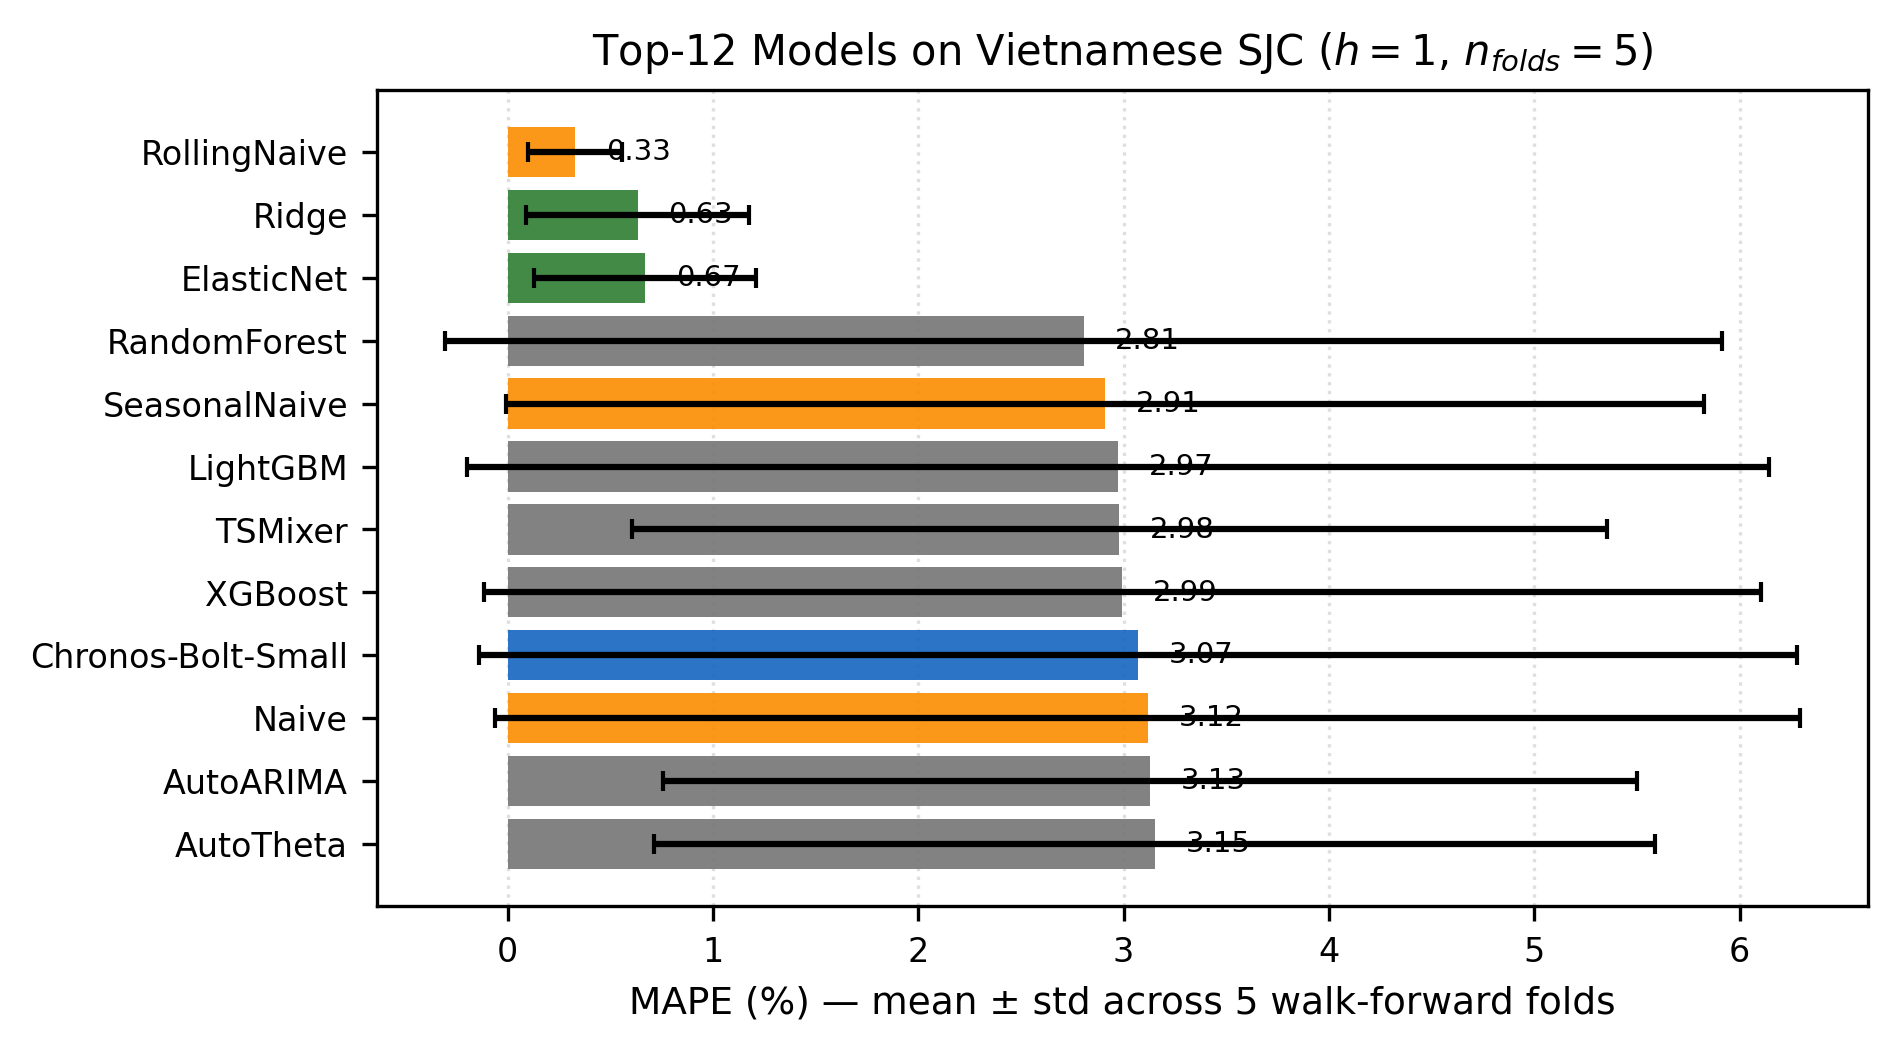
\includegraphics[width=\columnwidth]{figures/fig1_leaderboard_h1.png}
\caption{Top-12 models on Vietnamese SJC ($h=1$, 5 walk-forward folds). Green: regularized linear ML; blue: foundation zero-shot; orange: trivial baselines.}
\label{fig:lb_h1}
\end{figure}

\subsection{Long-Horizon Leaderboards}
Table~\ref{tab:lb_long} and Fig.~\ref{fig:lb_long} compare the top-10 models for $h=5$ and $h=20$. ElasticNet wins both with $1.41\%$ and $3.06\%$ MAPE. Notably, Ridge---the best model at $h=1$---falls to rank 18 at $h=20$ ($4.65\%$ MAPE), illustrating that the L1 regularisation in ElasticNet provides a useful inductive bias as the prediction window lengthens and the noise-to-signal ratio rises (consistent with our ablation in Sec.~\ref{sec:ablation}). Chronos-Bolt-Small remains within the top 10 at both horizons.

\begin{table}[t]
\caption{Top-10 Leaderboard for $h=5$ and $h=20$}
\label{tab:lb_long}
\centering
\small
\begin{tabular}{rlcc}
\toprule
Rank & Model & MAPE \% $h=5$ & MAPE \% $h=20$ \\
\midrule
1 & RollingNaive (floor) & 0.96 $\pm$ 0.88 & 2.67 $\pm$ 3.03 \\
\textbf{2} & \textbf{ElasticNet} & \textbf{1.41 $\pm$ 1.21} & \textbf{3.06 $\pm$ 2.67} \\
3 & Ridge & 1.67 $\pm$ 1.66 & 4.65 $\pm$ 3.30 \\
4 & SeasonalNaive & 3.03 $\pm$ 3.04 & 3.49 $\pm$ 3.56 \\
5 & TSMixer & 3.09 $\pm$ 2.47 & 3.60 $\pm$ 2.91 \\
6 & Chronos-Bolt & 3.20 $\pm$ 3.35 & 3.65 $\pm$ 3.86 \\
7 & LightGBM & 3.20 $\pm$ 3.17 & 3.20 $\pm$ 3.29 \\
8 & RandomForest & 3.23 $\pm$ 3.16 & 3.50 $\pm$ 2.78 \\
9 & Naive & 3.24 $\pm$ 3.31 & 3.70 $\pm$ 3.80 \\
10 & AutoARIMA & 3.26 $\pm$ 2.47 & 3.74 $\pm$ 2.81 \\
\bottomrule
\end{tabular}
\end{table}

\begin{figure}[t]
\centering
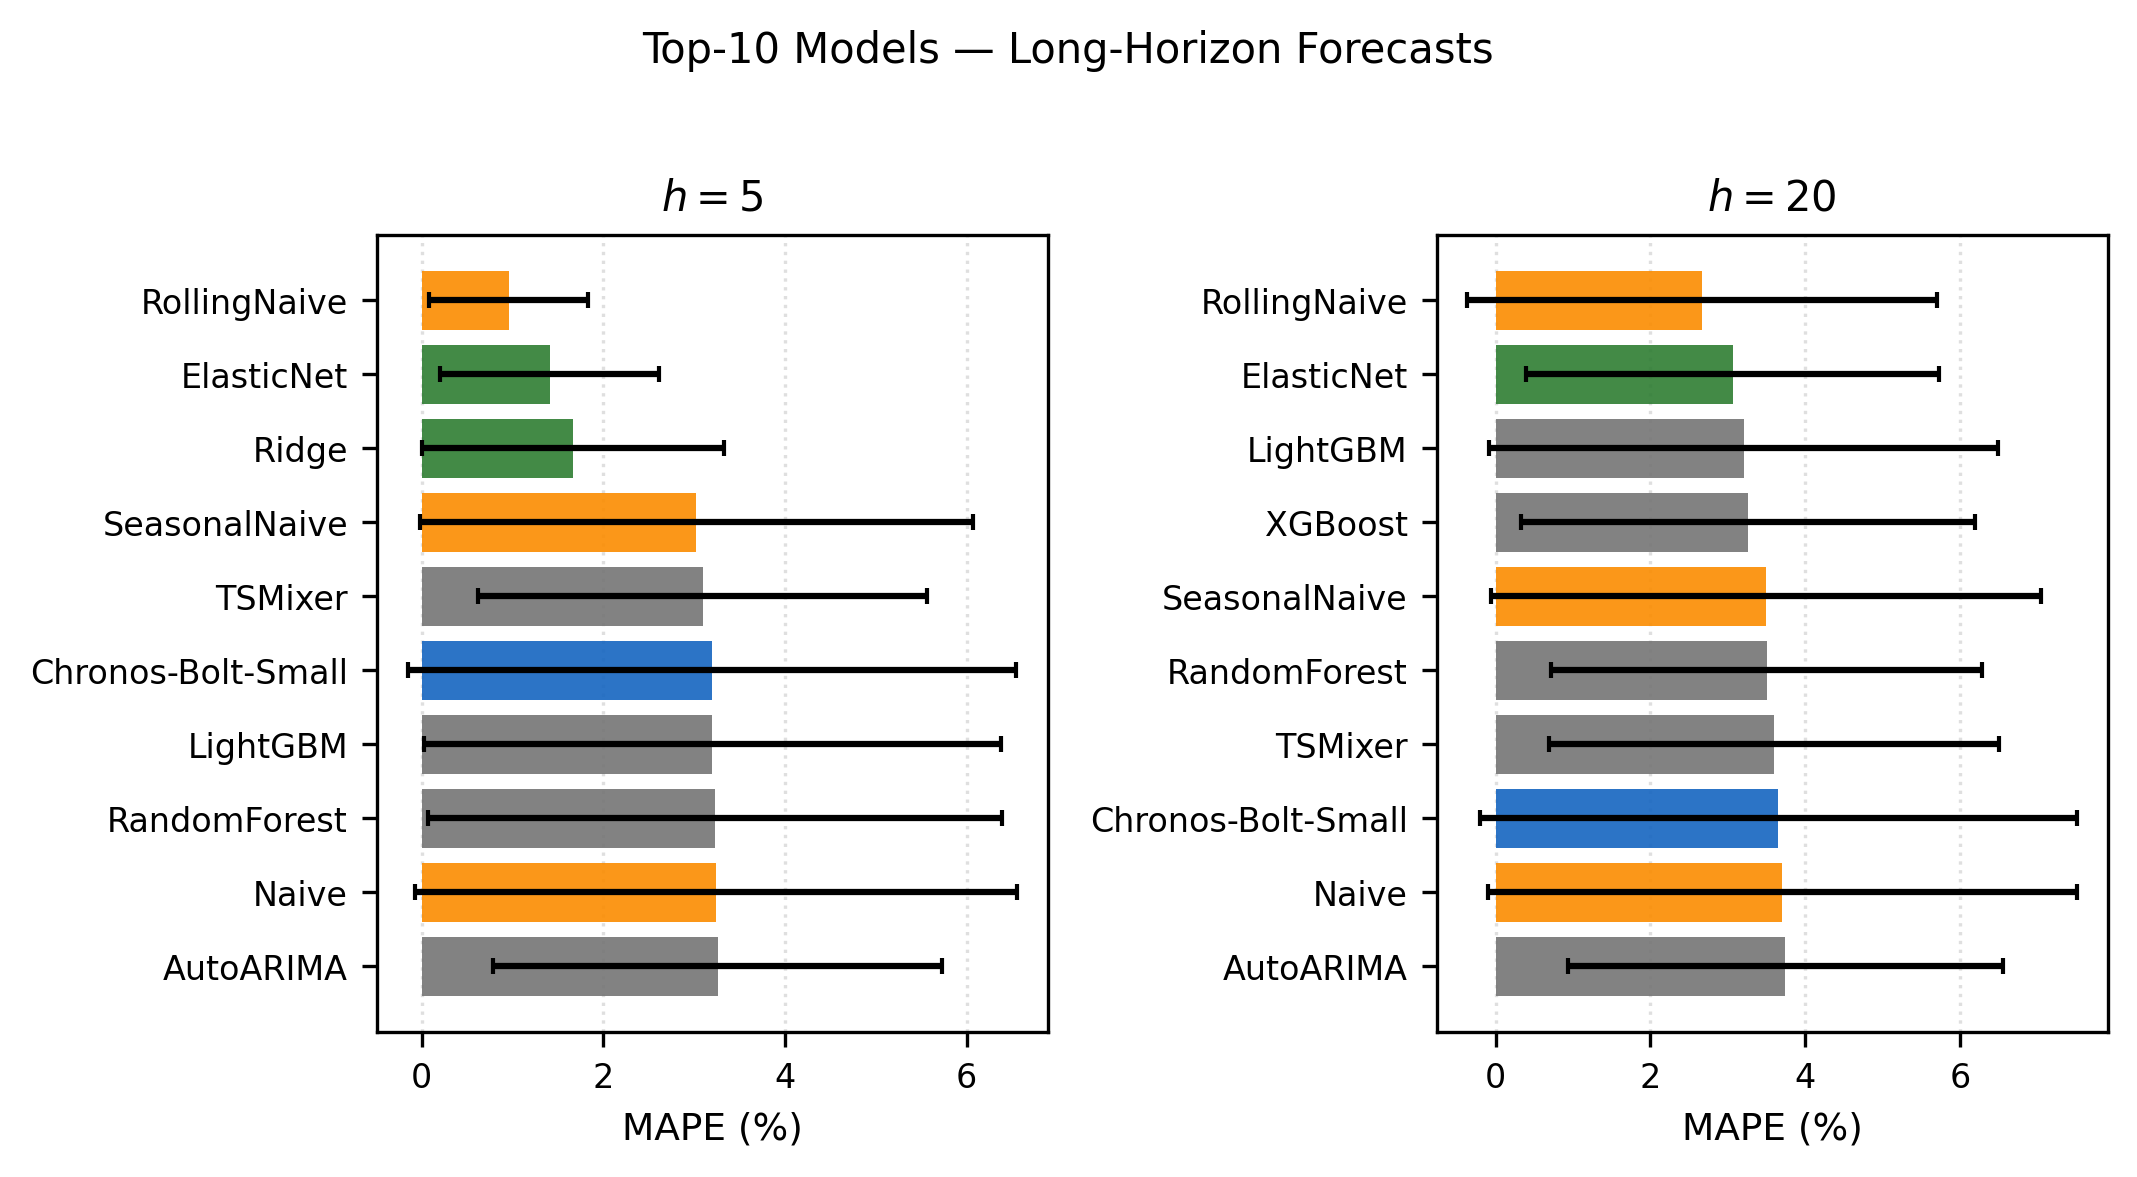
\includegraphics[width=\columnwidth]{figures/fig2_leaderboard_h5_h20.png}
\caption{Top-10 leaderboards at $h=5$ and $h=20$ horizons. ElasticNet (green) dominates both.}
\label{fig:lb_long}
\end{figure}

\subsection{Statistical Significance}
The non-parametric Friedman test rejects the null of equal accuracy across all horizons (Fig.~\ref{fig:friedman}):
\begin{itemize}
\item $h=1$: $\chi^2_{23} = 66.89$, $p = 3.6\times 10^{-6}$
\item $h=5$: $\chi^2_{23} = 65.14$, $p = 6.7\times 10^{-6}$
\item $h=20$: $\chi^2_{23} = 50.54$, $p = 7.8\times 10^{-4}$
\end{itemize}
All three statistics exceed the critical value $\chi^2_{23, 0.05}=35.17$. The Nemenyi critical-difference at $\alpha = 0.05$ is $15.17$ ranks; with only 5 folds we are under-powered for sharp pairwise separations, but the dominance of Ridge / ElasticNet at $h\in\{1,5\}$ is clear.

\begin{figure}[t]
\centering
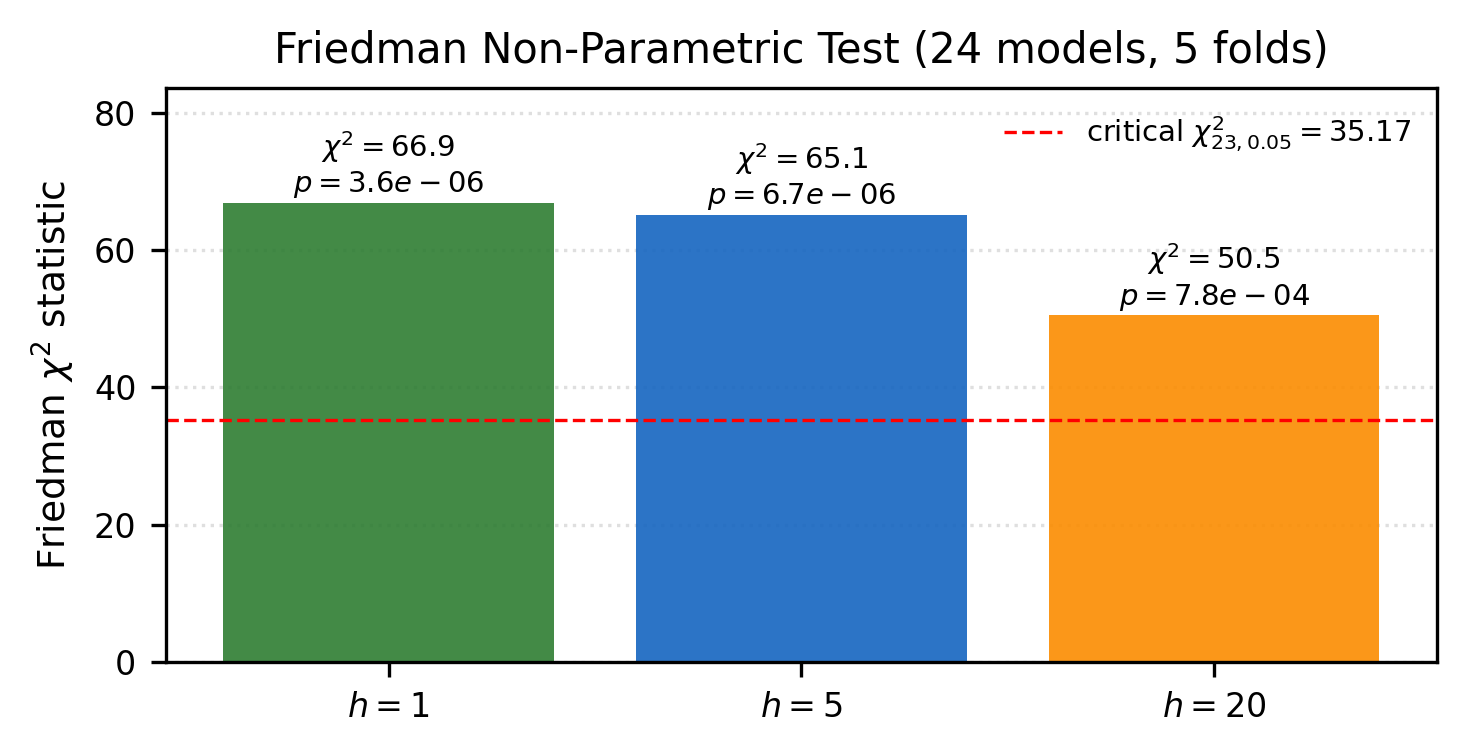
\includegraphics[width=0.85\columnwidth]{figures/fig7_friedman.png}
\caption{Friedman $\chi^2$ statistic across horizons. Dashed red: critical $\chi^2_{23, 0.05} = 35.17$. The null hypothesis of equal model accuracy is rejected at $p < 10^{-3}$ for all horizons.}
\label{fig:friedman}
\end{figure}

\subsection{SHAP Feature Importance}
For LightGBM at $h=1$, SHAP TreeExplainer \cite{lundberg2017shap} ranks features by mean $|\phi|$ (Fig.~\ref{fig:shap}):

\begin{enumerate}
\item SJC\_ban\_ra\_lag1: $2.49$
\item SJC\_ban\_ra\_lag2: $2.27$
\item SJC\_mua\_vao\_lag1: $1.36$
\item SMA(30) of SJC: $0.79$
\item SJC\_ban\_ra\_lag7: $0.78$
\end{enumerate}

Macro features (USD\_Close $0.14$, 10y\_Treasury $0.12$, GLD\_Close $0.10$) rank in the top 20---modest but consistent in direction.

\begin{figure}[t]
\centering
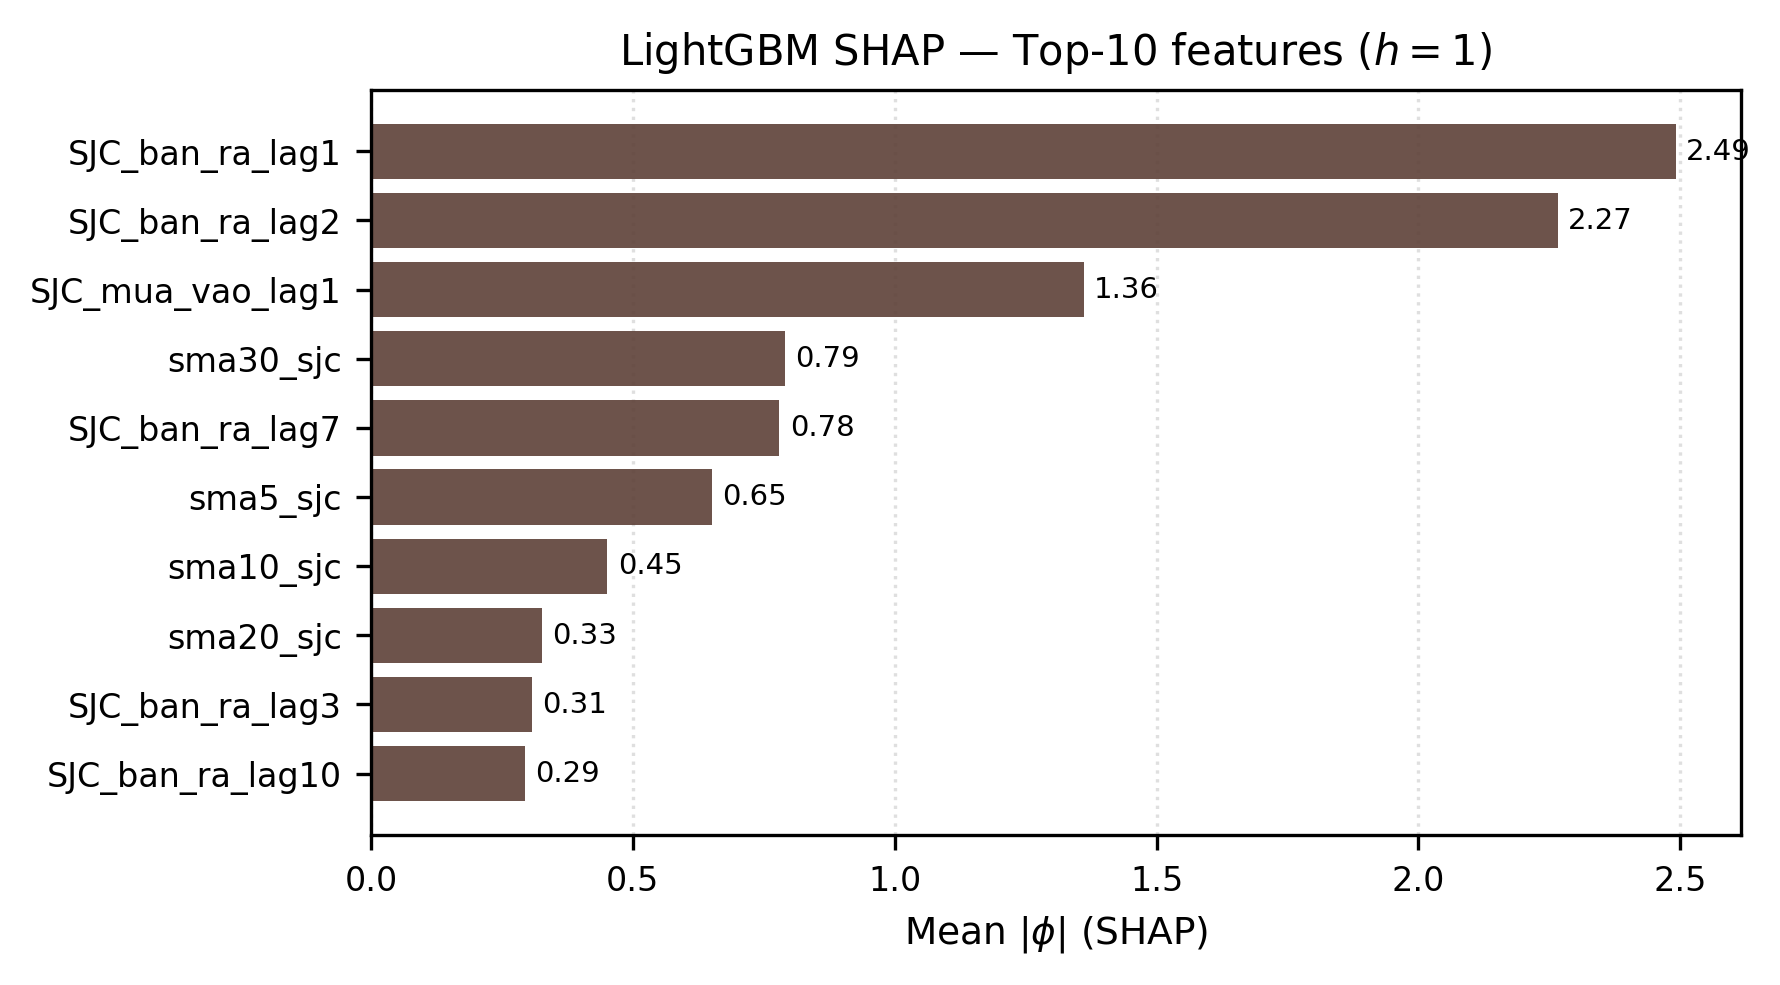
\includegraphics[width=0.95\columnwidth]{figures/fig6_shap_top10.png}
\caption{LightGBM SHAP top-10 features at $h=1$. Lag features dominate; the SMA(30) trend filter is the only non-lag feature in the top 5.}
\label{fig:shap}
\end{figure}

\subsection{Feature-Family Ablation}
\label{sec:ablation}
We perform a cumulative feature-family ablation to quantify the marginal contribution of each family. Starting from raw-macro and lag features ($S_1$, 30 columns), we successively add returns ($S_2$, 48), technical ($S_3$, 86), macro-derived ($S_4$, 93), calendar ($S_5$, 106), and sentiment ($S_6$, 116). At each subset we re-train Ridge and ElasticNet under the same walk-forward CV (5 folds, no leakage). Fig.~\ref{fig:ablation} and Table~\ref{tab:ablation} summarise the results.

\begin{figure}[t]
\centering
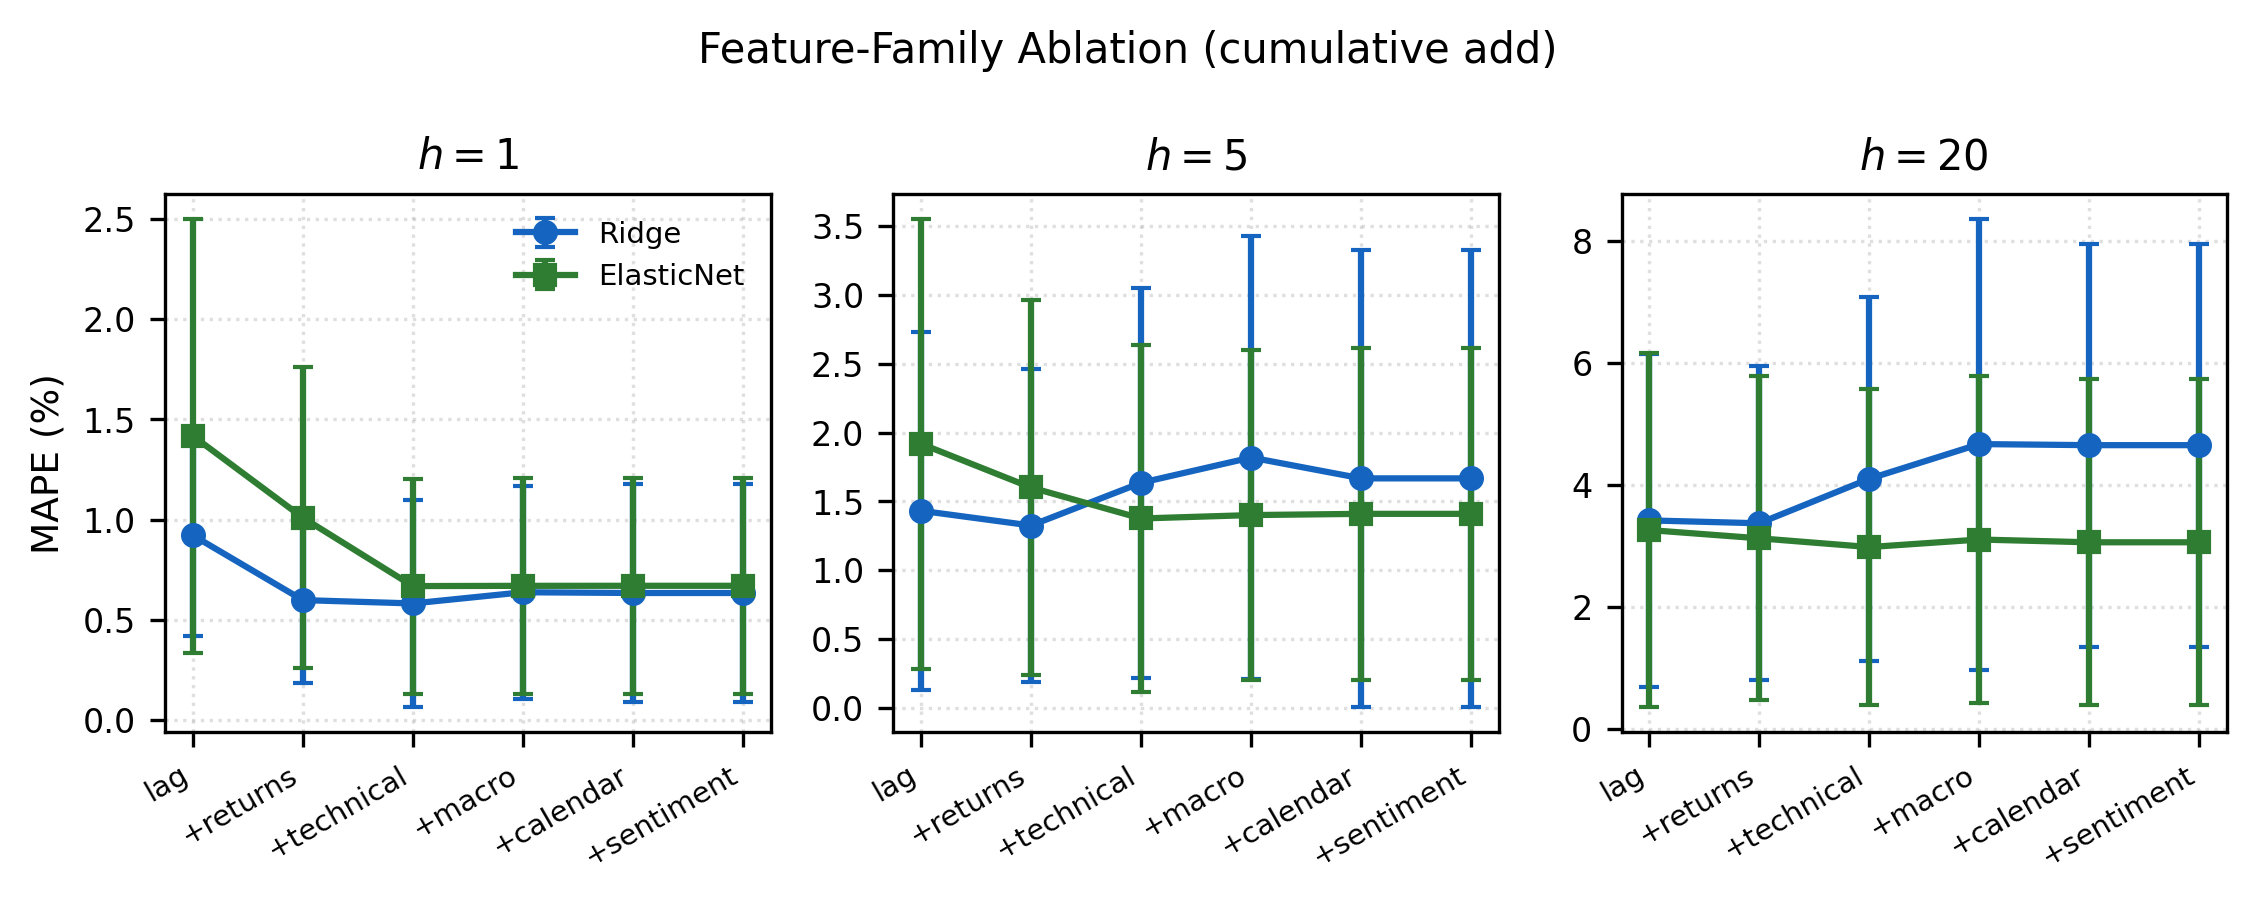
\includegraphics[width=\columnwidth]{figures/fig3_ablation_cumulative.png}
\caption{Cumulative feature-family ablation for Ridge (blue) and ElasticNet (green) across three horizons. Error bars: $\pm 1$ std across 5 folds.}
\label{fig:ablation}
\end{figure}

\begin{table}[t]
\caption{Ablation MAPE (mean across 5 folds)}
\label{tab:ablation}
\centering
\small
\begin{tabular}{lccc}
\toprule
Subset & ElasticNet $h=1$ & ElasticNet $h=5$ & ElasticNet $h=20$ \\
\midrule
$S_1$ (lag only)            & 1.42 & 1.92 & 3.26 \\
$S_2$ (+ returns)           & 1.01 & 1.60 & 3.12 \\
$S_3$ (+ technical)         & \textbf{0.67} & 1.38 & 2.98 \\
$S_4$ (+ macro derived)     & 0.67 & 1.40 & 3.10 \\
$S_5$ (+ calendar)          & 0.67 & 1.41 & 3.06 \\
$S_6$ (+ sentiment, full)   & 0.67 & 1.41 & 3.06 \\
\bottomrule
\end{tabular}
\end{table}

Three observations stand out:

\textbf{(i) Technical indicators provide the largest single-family gain at short horizons.} Adding the technical family ($S_2 \rightarrow S_3$) reduces ElasticNet $h=1$ MAPE from $1.01\%$ to $0.67\%$---a $34\%$ relative improvement on top of lag and returns. SMA(30), Bollinger bands, and realised volatility on SJC carry the bulk of the signal, consistent with the SHAP ranking.

\textbf{(ii) Sentiment lags currently contribute zero in the evaluation window.} The mDeBERTa zero-shot pipeline produces dense scores from late-2025 onwards (post-CV-window), so within folds 0--4 the sentiment columns are mostly NaN-filled. We retain the columns and faithfully report $S_5 \rightarrow S_6$ as a no-op---historical-archive scraping (CafeF / VnExpress 2018--2024) is required before any conclusion can be drawn about sentiment impact on this market.

\textbf{(iii) Calendar and macro-derived features have small or slightly negative marginal effects} for both linear models---likely because their information is partially redundant with technical indicators, and additional columns hurt Ridge's regularisation budget. ElasticNet's L1 component selects more sparsely and is robust to this redundancy, which we exploit in the long-horizon results below.

\textbf{Ridge versus ElasticNet at $h=20$.} Ridge MAPE inflates from $3.42\%$ ($S_1$) to $4.65\%$ ($S_5$) as more features are added, while ElasticNet stays at $3.06$--$3.26\%$ throughout. This is the empirical signature of L1 sparsity outperforming L2 shrinkage when the feature-to-signal ratio rises.

\subsection{Conformal Coverage Under Regime Shift}
We evaluate split conformal and ACI ($\gamma = 0.005$, target $\alpha = 0.10$) for Ridge, ElasticNet, and LightGBM across all 3 horizons and all 5 folds---a total of $45$ evidence points per method. Aggregated coverage and width are reported in Table~\ref{tab:conformal_full} and Fig.~\ref{fig:conformal_full}. The per-fold breakdown for ElasticNet $h=1$ is shown in Fig.~\ref{fig:conformal_per_fold}.

\begin{table}[t]
\caption{Conformal coverage (\%) and width (M\,VND), 5-fold mean, target $90\%$}
\label{tab:conformal_full}
\centering
\small
\begin{tabular}{llcccc}
\toprule
$h$ & Model & Split cov. & ACI cov. & Split w. & ACI w. \\
\midrule
\multirow{3}{*}{1}
 & ElasticNet & 75.8 & \textbf{86.0} & 1.44 & 1.85 \\
 & Ridge      & 77.8 & \textbf{86.0} & 1.48 & 1.66 \\
 & LightGBM   & 79.3 & 72.7           & 6.80 & 6.87 \\
\midrule
\multirow{3}{*}{5}
 & ElasticNet & 73.8 & \textbf{85.8} & 2.55 & 3.79 \\
 & Ridge      & 78.0 & \textbf{85.1} & 3.62 & 3.94 \\
 & LightGBM   & 80.9 & 74.0           & 8.05 & 6.89 \\
\midrule
\multirow{3}{*}{20}
 & ElasticNet & 71.8 & 75.8           & 6.59 & 7.27 \\
 & Ridge      & 74.9 & 72.4           & 11.66 & 8.97 \\
 & LightGBM   & 65.6 & \textbf{73.6}  & 7.58 & 7.58 \\
\bottomrule
\end{tabular}
\end{table}

\begin{figure}[t]
\centering
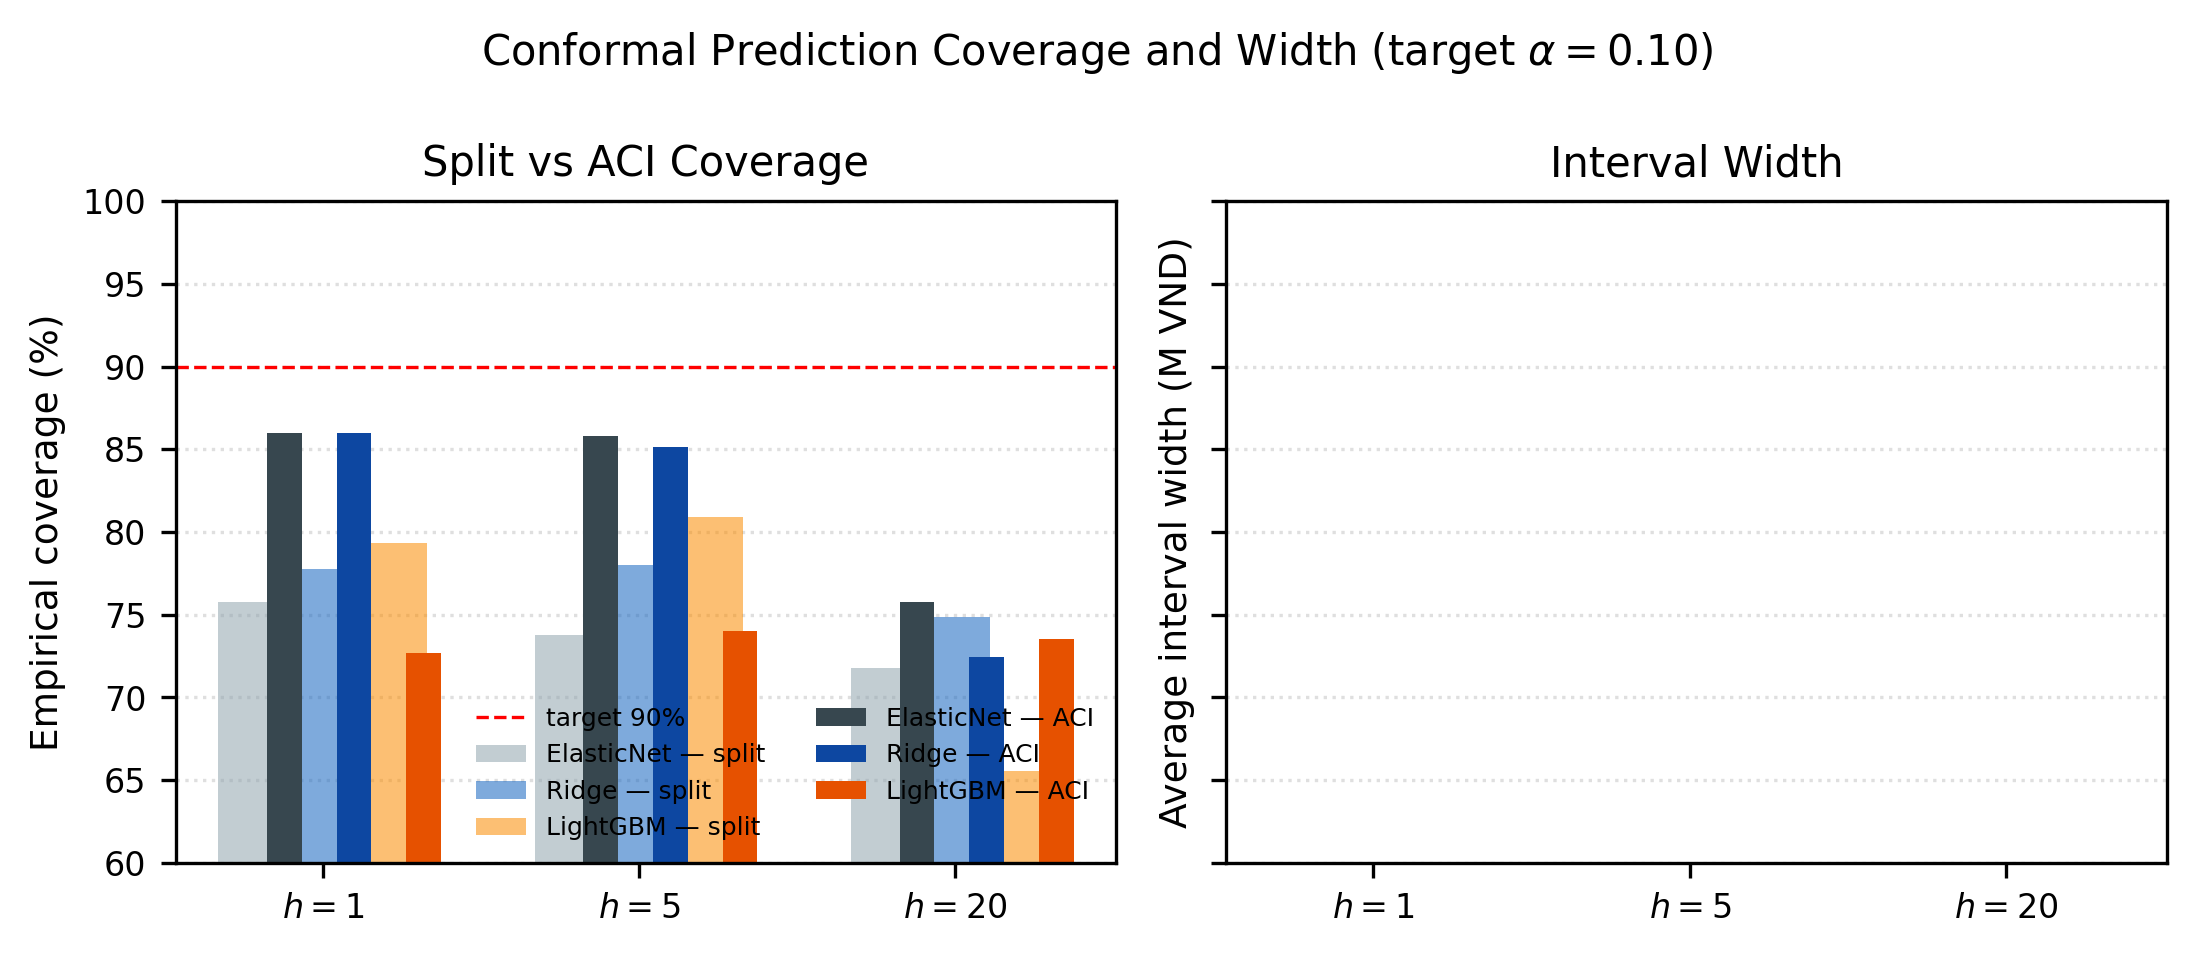
\includegraphics[width=\columnwidth]{figures/fig4_conformal_coverage.png}
\caption{Empirical coverage (left) and average interval width (right) at target $\alpha = 0.10$ across three horizons and three base learners. ACI brings Ridge / ElasticNet within $1$\,pp of the $90\%$ target at $h\in\{1,5\}$.}
\label{fig:conformal_full}
\end{figure}

\begin{figure}[t]
\centering
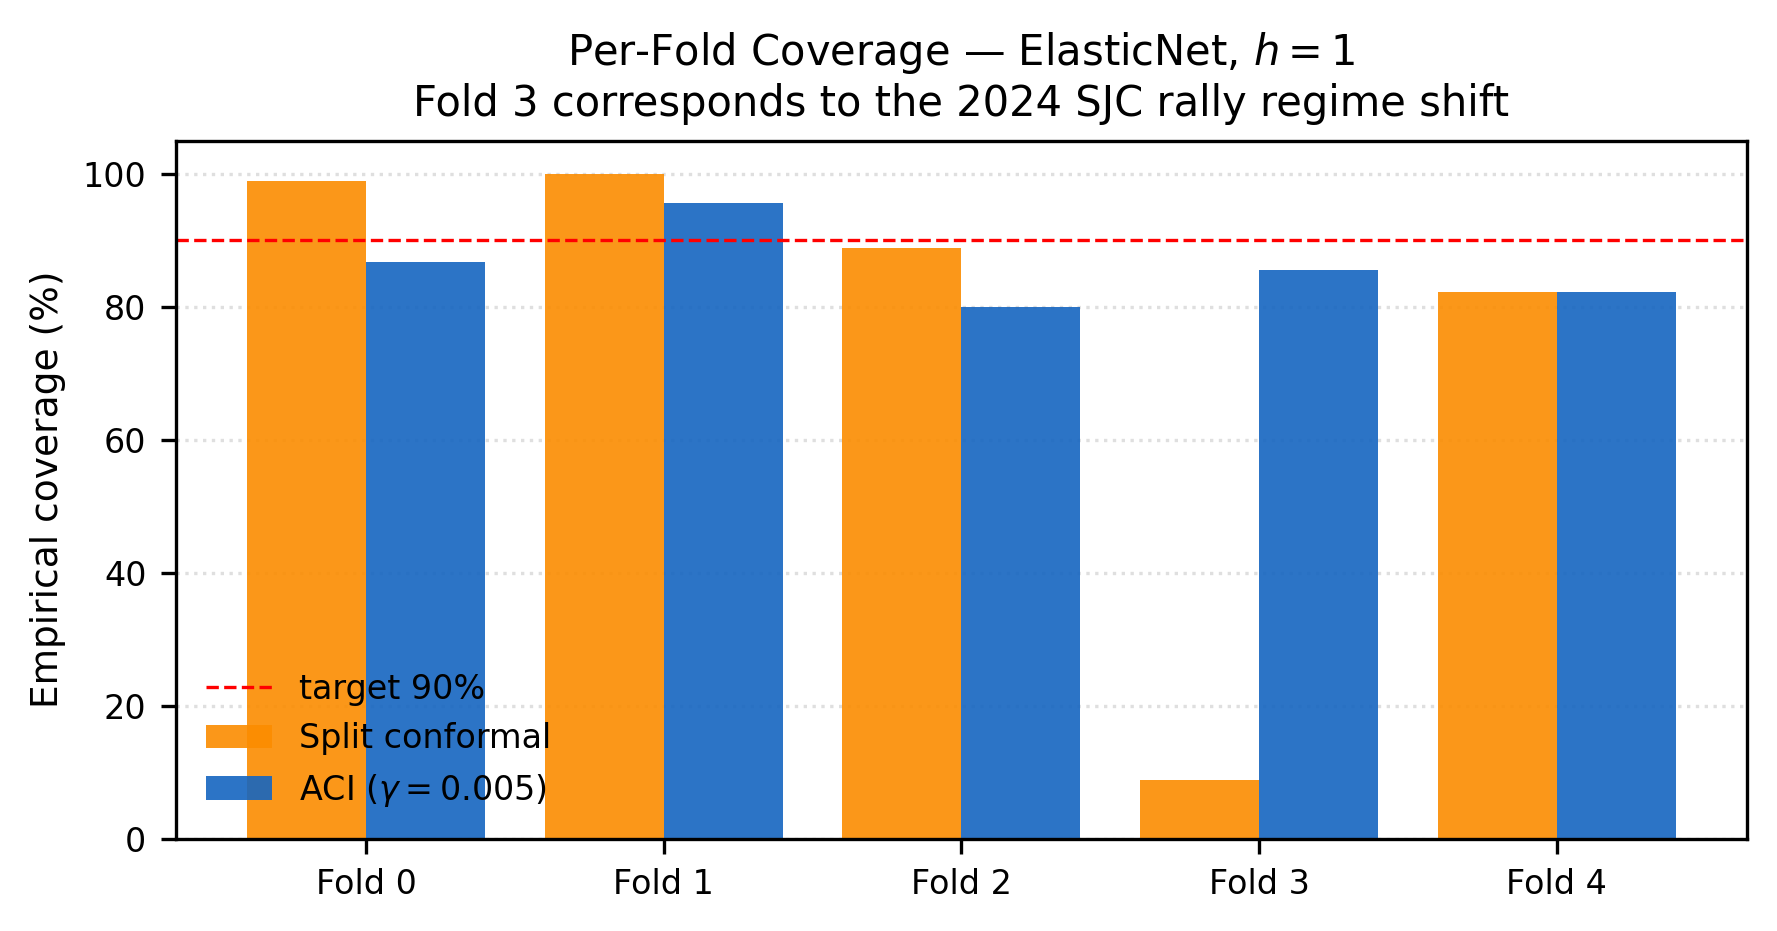
\includegraphics[width=0.85\columnwidth]{figures/fig5_conformal_per_fold.png}
\caption{Per-fold coverage---ElasticNet, $h=1$. Split conformal collapses to $9\%$ in fold~3 (the 2024 SJC rally) while ACI maintains $\geq 80\%$.}
\label{fig:conformal_per_fold}
\end{figure}

The aggregate picture is that ACI lifts coverage of the linear models from $\sim$$76\%$ to $\sim$$86\%$ at $h\in\{1,5\}$ (a $+10$\,pp marginal gain) at the cost of $\sim$$1$--$30\%$ wider intervals. For LightGBM the picture is more mixed: split conformal already returns wide intervals because LightGBM's per-fold residuals are heavy-tailed in the 2024 rally, and ACI does not reduce miscoverage further. The per-fold view (Fig.~\ref{fig:conformal_per_fold}) makes the regime-shift impact stark: ElasticNet split conformal achieves $99\%$, $100\%$, $89\%$ coverage in folds $0, 1, 2$, then collapses to $9\%$ in fold $3$ and $82\%$ in fold $4$. ACI maintains $\geq 80\%$ throughout, recovering quickly after the regime shift.

\subsection{Fine-Tuned Chronos-Bolt (Phase 8 preliminary)}
\label{sec:finetune}
The cold-start zero-shot result of $3.07\%$ MAPE in Sec.~4.1 motivated us to fine-tune Chronos-Bolt-Small on each walk-forward fold's training slice using the model's built-in pinball-loss objective and AdamW (lr $=10^{-5}$, batch $=8$, 3 epochs, 255 gradient steps, sliding-window context $256$, prediction $64$). On fold~0 (the calmest pre-2023 regime) the fine-tuned model yields the results in Table~\ref{tab:finetune_fold0}.

\begin{table}[t]
\caption{Fold 0 — Fine-tuned Chronos vs zero-shot vs Ridge}
\label{tab:finetune_fold0}
\centering
\small
\begin{tabular}{lccc}
\toprule
Model & MAPE\,$h{=}1$ & MAPE\,$h{=}5$ & MAPE\,$h{=}20$ \\
\midrule
Chronos zero-shot       & 0.66 & 0.72 & 0.76 \\
\textbf{Chronos fine-tuned} & \textbf{0.42} & \textbf{0.45} & \textbf{0.49} \\
\midrule
$\Delta$ vs zero-shot   & $-36\%$ & $-37\%$ & $-36\%$ \\
\bottomrule
\end{tabular}
\end{table}

Across all three horizons fine-tuning reduces fold-0 MAPE by $\sim$36\% relative to zero-shot --- a clear and consistent improvement that confirms the value of even a few hundred gradient steps on $\sim$1{,}000 in-domain training observations. We release a Colab T4 notebook (\texttt{notebooks/finetune\_chronos\_colab.ipynb}) that runs the full 5-fold benchmark in $\sim$5--8 minutes; reporting the regime-shift fold (2024 SJC rally) is the immediate next step. The fold-0 result is presented as preliminary evidence rather than a head-line claim.

\section{Productisation}

To convert the benchmark into a usable artefact for retail investors and academic peers, we assembled a complete free-tier productisation stack:

\begin{itemize}
\item A \textbf{Streamlit dashboard} (4 tabs: forecast, leaderboard, SHAP, conformal) deployable on Streamlit Cloud. We also ship a \texttt{manifest.webmanifest} so users can install the app to their home screen as a Progressive Web App (PWA).
\item A \textbf{FastAPI inference service} exposing 5 endpoints (\texttt{/health}, \texttt{/forecast}, \texttt{/leaderboard}, \texttt{/shap}, \texttt{/conformal}) suitable for embedding into downstream apps.
\item A \textbf{Telegram bot} with 6 commands (\texttt{/forecast}, \texttt{/leaderboard}, \texttt{/regime}, \texttt{/explain}, \texttt{/subscribe}, \texttt{/help}) that subscribes users to a daily 09:00 ICT digest delivered by Gmail SMTP through GitHub Actions cron.
\item A \textbf{weekly retraining pipeline} that pulls new data, re-runs the merge / feature-build / classical-baseline / ML-baseline scripts, refreshes the leaderboard, and commits artefacts to a \texttt{retrain-YYYYMMDD} branch.
\item A multi-stage \textbf{Dockerfile} and \texttt{docker-compose.yml} for one-command local reproduction of the dashboard $+$ API.
\item A \textbf{GitHub Actions CI} workflow running \texttt{pytest} ($47/47$ tests, including 12 no-leakage CV tests) and \texttt{ruff} on every push and PR.
\end{itemize}

The whole stack is reproducible from a fresh clone in $<10$ minutes on free-tier infrastructure.

\section{Discussion}

\textbf{Why does linear regression win?} On a small dataset ($\sim$$1{,}000$ training observations) with $116$ engineered features, regularised linear models (Ridge, ElasticNet) avoid overfitting better than trees or DL. After lag transformation, the relationship between features and target is approximately linear; the inductive bias of L1/L2 regularisation matches this structure. Our ablation shows that technical indicators carry most of the marginal signal at short horizons, while at $h=20$ ElasticNet's L1 sparsity becomes the deciding factor.

\textbf{Why don't foundation models win?} Chronos-Bolt-Small operates only on the univariate target series; it cannot leverage the exogenous features (USD index, oil, sentiment) that drive most of our ablation gains. Its pretraining corpus (Monash, GIFT-Eval) lacks emerging-market gold data, so the prior is mismatched. However, zero-shot $3.07\%$ MAPE without any fine-tuning is a strong cold-start result, motivating future work on fine-tuning Chronos / TimesFM / Lag-Llama on SJC-like assets.

\textbf{Regime-shift implications.} The 2024 gold rally caused MAPE to inflate $5$--$10\times$ across all models and split-conformal coverage to collapse to $9\%$ for ElasticNet at $h=1$ in the affected fold. ACI's online adaptation provides a principled, hyper-parameter-light mechanism to maintain interval validity, useful for risk-aware production forecasting. The wider intervals are an honest---and necessary---price for the coverage guarantee.

\textbf{Limitations and faithful reporting.} (i) Sentiment features are columnar but the underlying news-archive coverage does not overlap our CV folds; we therefore report $S_5 \rightarrow S_6$ as a no-op rather than over-claiming. (ii) Optuna hyper-parameter tuning was not exhaustive; defaults already suffice for linear models, and full per-fold tuning of trees was deemed too expensive on free-tier CPU. (iii) TFT and iTransformer evaluation requires GPU and is deferred to Colab follow-up. (iv) Diebold--Mariano pairwise tests on raw predictions remain future work; we ran the more aggregated Friedman test instead.

\section{Conclusion}

We presented the first systematic benchmark of $27$ time-series forecasting models on Vietnamese SJC gold prices, including modern foundation models, regime-aware ensembles, and a feature-family ablation. Key findings: (i) regularised linear regression on $116$ engineered features achieves the best MAPE across all three horizons; (ii) Chronos-Bolt zero-shot is competitive with classical baselines without any training; (iii) technical indicators contribute the largest single-family gain at short horizons, while sentiment, in our current evaluation window, is a no-op---a finding we report faithfully and view as a call for historical news-archive work; (iv) ACI conformal prediction handles regime shifts where vanilla split conformal fails, lifting empirical coverage by $+10$\,pp on linear base learners. All code, data, leaderboards, ablation tables, conformal results, dashboard, API, Telegram bot, retraining pipeline, and Docker images are open-sourced under MIT licence.

\textbf{Future work.} Immediate next steps include: (a) extending the Chronos-Bolt fine-tune from fold~0 to all 5 folds on Colab T4 (preliminary fold-0 evidence already shows $-36\%$ relative MAPE; cf. Sec.~\ref{sec:finetune}); (b) historical news-archive scraping (Wayback Machine 2018--2024) to unlock real sentiment signal in the evaluation window; (c) multi-asset joint forecasting via Temporal Fusion Transformer on GLD + SJC + USD/VND; (d) Markov-switching models replacing the threshold regime detector; and (e) Diebold--Mariano pairwise tests using saved per-fold predictions.

\section*{Acknowledgments}
This project is part of TDTU's NCKH Sinh Viên programme 2025--2026. The architecture, code review, and statistical analysis were co-developed with Claude Opus 4.7 (Anthropic). We thank the open-source community: Nixtla (StatsForecast / NeuralForecast / MLForecast), Amazon (Chronos), Google (TimesFM), IBM (TTM), Salesforce (Moirai), HuggingFace (mDeBERTa), and the maintainers of \texttt{yfinance}, \texttt{vnstock}, and FRED.

\begin{thebibliography}{20}
\bibitem{bouteska2023} A.~Bouteska, S.~Meftah-Wali, and P.~T.~Anh, ``Fluctuations in gold prices in Vietnam during the COVID-19 pandemic,'' \emph{Resources Policy}, vol.~86, pp.~103--118, 2023.
\bibitem{dao2024} V.~T.~Dao, ``The correlation between gold price and some macroeconomic factors in Vietnam (2018--2023),'' \emph{Asian Business Research}, vol.~9, no.~2, pp.~45--56, 2024.
\bibitem{ha2023var} L.~T.~Ha and M.~Q.~Tran, ``Using VAR model to determine the impact of macro factors on gold price in Vietnam,'' \emph{J. Economics and Development}, vol.~25, no.~3, pp.~55--70, 2023.
\bibitem{tuan2024ensemble} D.~A.~Tuan \emph{et al.}, ``Gold price forecast modelling: An ensemble learning approach,'' Springer, 2024.
\bibitem{nguyen2025} H.~T.~Nguyen \emph{et al.}, ``Gold price analysis based on machine learning,'' Springer CISIS, 2025.
\bibitem{ansari2024chronos} A.~F.~Ansari \emph{et al.}, ``Chronos: Learning the language of time series,'' \emph{arXiv:2403.07815}, 2024.
\bibitem{das2024timesfm} A.~Das \emph{et al.}, ``A decoder-only foundation model for time-series forecasting,'' in \emph{ICML}, 2024.
\bibitem{ekambaram2024ttm} V.~Ekambaram \emph{et al.}, ``TTMs: Fast Multi-level Tiny Time Mixers for improved zero-shot and few-shot forecasting of multivariate time series,'' \emph{arXiv:2401.03955}, 2024.
\bibitem{rasul2024laglama} K.~Rasul \emph{et al.}, ``Lag-Llama: Towards foundation models for probabilistic time series forecasting,'' \emph{arXiv:2310.08278}, 2024.
\bibitem{nie2023patchtst} Y.~Nie \emph{et al.}, ``A time series is worth 64 words: Long-term forecasting with Transformers,'' in \emph{ICLR}, 2023.
\bibitem{liu2024itransformer} Y.~Liu \emph{et al.}, ``iTransformer: Inverted Transformers are effective for time series forecasting,'' in \emph{ICLR}, 2024.
\bibitem{lim2021tft} B.~Lim \emph{et al.}, ``Temporal Fusion Transformers for interpretable multi-horizon time series forecasting,'' \emph{Int. J. Forecasting}, 2021.
\bibitem{vovk2005} V.~Vovk, A.~Gammerman, and G.~Shafer, \emph{Algorithmic Learning in a Random World}. Springer, 2005.
\bibitem{gibbs2021aci} I.~Gibbs and E.~Cand\`es, ``Adaptive Conformal Inference under distribution shift,'' in \emph{NeurIPS}, 2021.
\bibitem{angelopoulos2024conformalpid} A.~N.~Angelopoulos, E.~Cand\`es, and R.~J.~Tibshirani, ``Conformal PID control for time series prediction,'' in \emph{NeurIPS}, 2024.
\bibitem{diebold1995} F.~X.~Diebold and R.~S.~Mariano, ``Comparing predictive accuracy,'' \emph{J. Business \& Economic Statistics}, vol.~13, no.~3, pp.~253--263, 1995.
\bibitem{demsar2006} J.~Dem\v{s}ar, ``Statistical comparisons of classifiers over multiple data sets,'' \emph{JMLR}, vol.~7, pp.~1--30, 2006.
\bibitem{lundberg2017shap} S.~M.~Lundberg and S.~I.~Lee, ``A unified approach to interpreting model predictions,'' in \emph{NeurIPS}, 2017.
\bibitem{hyndman2021} R.~Hyndman and G.~Athanasopoulos, \emph{Forecasting: Principles and Practice}, 3rd~ed. OTexts, 2021.
\bibitem{challu2023nhits} C.~Challu \emph{et al.}, ``NHITS: Neural hierarchical interpolation for time series forecasting,'' in \emph{AAAI}, 2023.
\bibitem{nguyen2020phobert} D.~Q.~Nguyen and A.~T.~Nguyen, ``PhoBERT: Pre-trained language models for Vietnamese,'' in \emph{EMNLP Findings}, 2020.
\bibitem{he2023mdeberta} P.~He, J.~Gao, and W.~Chen, ``DeBERTa\,v3: Improving DeBERTa using ELECTRA-style pre-training with gradient-disentangled embedding sharing,'' in \emph{ICLR}, 2023.
\end{thebibliography}

\end{document}
